% Template for Cogsci submission with R Markdown

% Stuff changed from original Markdown PLOS Template
\documentclass[10pt, letterpaper]{article}

\usepackage{cogsci}
\usepackage{pslatex}
\usepackage{float}
\usepackage{caption}

% amsmath package, useful for mathematical formulas
\usepackage{amsmath}

% amssymb package, useful for mathematical symbols
\usepackage{amssymb}

% hyperref package, useful for hyperlinks
\usepackage{hyperref}

% graphicx package, useful for including eps and pdf graphics
% include graphics with the command \includegraphics
\usepackage{graphicx}

% Sweave(-like)
\usepackage{fancyvrb}
\DefineVerbatimEnvironment{Sinput}{Verbatim}{fontshape=sl}
\DefineVerbatimEnvironment{Soutput}{Verbatim}{}
\DefineVerbatimEnvironment{Scode}{Verbatim}{fontshape=sl}
\newenvironment{Schunk}{}{}
\DefineVerbatimEnvironment{Code}{Verbatim}{}
\DefineVerbatimEnvironment{CodeInput}{Verbatim}{fontshape=sl}
\DefineVerbatimEnvironment{CodeOutput}{Verbatim}{}
\newenvironment{CodeChunk}{}{}

% cite package, to clean up citations in the main text. Do not remove.
\usepackage{cite}

\usepackage{color}

% Use doublespacing - comment out for single spacing
%\usepackage{setspace}
%\doublespacing


% % Text layout
% \topmargin 0.0cm
% \oddsidemargin 0.5cm
% \evensidemargin 0.5cm
% \textwidth 16cm
% \textheight 21cm

\title{Optimal Models for Resource Allocation in Classroom Education}


\author{{\large \bf Larry Liu} \\ \texttt{hrlarry@stanford.edu} \\ Department of Psychology \\ Stanford University \And {\large \bf Michael C. Frank} \\ \texttt{mcfrank@stanford.edu} \\ Department of Psychology \\ Stanford University}

\begin{document}

\maketitle

\begin{abstract}
Education is the transmission of knowledge from teacher to student.
\textbf{FIXME}: How should a school administrator allocate a fixed
budget towards increasing the number of classrooms and increasing
student assessment to best increase student learning? This paper
investigates how stochastic models accounting for the inherent
uncertainty in student beliefs and teacher communication in
teacher-student dyads can help school administrators figure out how to
maximize student learning by optimally allocating resources. We
replicate existing results from edu- cation literature about the effect
of class sizes, homogenous ability classrooms, and assessment on student
learning using computer simulation. We also unify these different
determi- nants of student learning into a more holistic model and report
the tradeoffs that committing budget to these design features presents.
We demonstrated that we can create a pareto frontier for the number of
teachers and assessments against a fixed bud- get, and find an optimal
allocation of the budget for increasing student learning. We also
demonstrate how the effectiveness of class sizes and assessment is
contingent upon the learning concept being taught. We believe that the
insights about stu- dent learning in multi-classroom settings that we've
found and can continue to surface are difficult to surface in real-world
studies with human subjects.

\textbf{Keywords:}
Teaching; learning; education; pragmatics; Bayesian modeling; social
cognition
\end{abstract}

Education is the process of knowledge transmission from teachers to
students. A teacher attempts to provide information to students --
whether facts, skills, generalizations, or another type of knowledge --
in a form that will be most likely to result in the student learning.
But even when students are motivated to learn, and teachers are
motivated to teach, information transmission in the classroom is
imperfect. Classroom teachers must teach to students with different
abilities and backgrounds, making the perfect lesson for one child less
accessible to another (the problem of \emph{student variability}).
Adding to this issue, teachers don't have perfect knowledge of what
students know or how they learn (the problem of \emph{imperfect
knowledge}).

Educators have a variety of tools to address these problems. If students
are too diverse in their knowledge, they can be grouped by ability and
provided with different lessons (e.g., Slavin, 1987; Tomlinson, 1999).
And formative assessments -- tests that reveal a student's starting
state -- can help teachers know what level students start at (L. S.
Fuchs \& Fuchs, 1986; e.g., Sadler, 1989). But breaking students up into
groups or separate classes is resource intensive and can be inefficient
-- in the limit, it would be impossible to give every single student a
separate tutor, even if it might learn to better learning. And every
assessment has a cost in terms of lost instructional time. When should
educators use these tools? The goal of the current paper is to provide a
formal analysis of these questions.

In our previous work, we conceptualized the teacher's task as one of
optimal communication (Frank, 2014). Following models of pragmatic
reasoning in langauge comprehension (Frank \& Goodman, 2012; Goodman \&
Frank, 2016), we modeled teachers as reasoning about what evidence would
best change student beliefs to more closely correspond to a target.
Teachers -- with perfect knowledge about each of their students -- would
then choose the learning example that maximized information gain across
their students. Using this conceptualization, we were able to derive a
number of results through simulation. For example, we found that
individual student outcomes were inversely related to class size, since
in smaller classes, teachers could customize their teaching better to
the idiosynrasies of their particular student group.\footnote{Ability
  grouping has a complicated history in education (e.g., Slavin, 1990),
  and we return to motivational issues related to this finding in the
  General Discussion.}

In that previous work and the current work, the fundamental unit of
analysis is a teaching game. In each teacher-student dyad, a teacher
tries to guide the student to discover a particular concept by
presenting examples. We use a very simple concept, the weight of a
biased coin (i.e., the parameter of a Bernoulli distribution, from
0--1). For this concept, teaching lessons are the results of individual
coin flips, which provide evidence about the coin's weight. Beliefs can
then be represented as the parameters of a Beta distribution. For
example, a student who has a weak belief that a coin is fair (e.g.,
\(Beta(1,1)\)) can be pursuaded that it is actually biased towards heads
by seeing the examples \(E = \{H, H, H, H, H\}\). Despite the simplicity
of this teaching game, when analyzed at the level of multiple students
and multiple teachers, it reveals many interesting dynamics.

In the current work, we consider issues of student variability and
imperfect teacher knowlege through the lens of \emph{optimal school
administration}. Given finite resources, what arrangement of teachers
and students, and assessements and lessons, produces the greatest
information gain? We describe a generalization of the model presented in
Frank (2014) and use this framework to investigate how an optimal
adminstrator might make decisions. Our first two simulations replicate
and extend results from the previous paper. Then our next two generalize
the model to the case of imperfect information about students and finite
resources for hiring teachers and conducting assessments. Our final
simulation maps out a Pareto frontier for allocation of instructional
time and teaching resources. Taken together, this work describes a
first-principles attempt at a framework for understanding resource
allocation in classroom education.

\section{Model}\label{model}

We model three types of agents: \emph{students}, \emph{teachers}, and
\emph{administrators}. A school consists of an administrator, at least
one teacher, and at least one student. Every teacher has at least one
student (so there are always at least as many teachers as students).
Each agent's functions are described below.

\subsection{Student}\label{student}

Each student is an optimal Bayesian learner of a coin weight, using a
standard conjugate Beta-Bernoulli model. Students have a \emph{prior
belief} about the bias of the coin, represented as
\(Beta(\alpha,\beta)\), where \(\alpha\) and \(\beta\) are
``pseudo-counts'' (they can be interpreted as \(H\)=heads=1 and
\(T\)=tails=0 coin flips that the student has previously seen). Student
beliefs are drawn by sampling \(\alpha \sim Unif(1,10)\) and then
setting \(\beta = 11 - \alpha\) (so that total pseudocounts sum to 11).
Students' learning is then modeled as updating this distribution by
adding observed counts to their priors, e.g.~after observing \(x\) heads
and \(y\) tails, their updated knowledge state is
\(Beta(\alpha + x, \beta + y)\). Note that for simplicity, student
learning is sequence-independent (i.e., seeing \(\{H, T, T\}\) is the
same as seeing \(\{T, T, H\}\)).

\subsection{Teacher}\label{teacher}

Each teacher is assigned a classroom of students and a target concept
(i.e., a particular coin weight) to teach. The goal of the teacher is to
provide the set of examples that maximize the student's information gain
(IG; defined below). This goal is accomplished by evaluating the
information gain for each student for each possible example set and
choosing the one that produces the largest total information gain for
the class.\footnote{A fruitful direction for future work would be to
  investigate different classroom rules for information gain. For
  example, a teacher following a remedial policy could try to find the
  set of examples that maximized the performance of the
  lowest-performing students or that minimized loss with respect to some
  threshold.} Since information gain is computed over the conjugate
posterior representation of student knowledge, choosing an action
relative to IG constitutes full posterior inference. With only a single
teaching example, this choice is simply the ratio of the IG for \(H\) to
the IG for \(T\).

\textbf{TODO: change here if simulation numbering changes} In
Simulations 1 and 2, teachers have \emph{perfect knowledge} of student
beliefs. Teachers with perfect knowledge infer their choice of examples
using the exact parameters of student distributions. In contrast, the
teachers in the remaining simulations have \emph{uncertain knowledge}.
Teachers with uncertain knowledge initially represent students as having
beliefs in the form of \(Beta(1,1)\) -- weak uniform distributions over
possible parameter values. They update these representations based on
\emph{assessments}. Assessments are sampled examples from each student's
mean parameter estimate, using \(\mu = \frac{\alpha}{\alpha + \beta}\).
Teachers integrate the samples from these assessments into their
distributional estimate for each student. For example, if a student was
given three assessments and produced \(\{H, T, H\}\), the teacher would
represent that student as \(Beta(1+2,1+1) = Beta(3,2)\) and choose
examples to accordingly.

\subsection{Administrator}\label{administrator}

The objective of the administrator is to maximize the information gain
of all students in the school. Across our simulations, the administrator
can decide: 1) how many teachers to hire, 2) how many assessments to
give, and 3) whether to sort students into classrooms by their
knowledge. We also vary (for purposes of comparison) whether the
teachers have perfect or uncertain knowledge of the students. The
administrator weights the various policies that they simulate based on
the aggregate information gain of the students in the entire school
(compared to just each classroom for each teacher's inference), and is
able to infer the most effective school design within fixed constraints.

The administrator's main constraint is on assessment: each assessment
takes the same ``time'' as a teaching example. This constraint
represents the idea that there is a cost in terms of instruction time
for getting information about students via assessment. Of course, the
exact ratio of costs is an arbitrary parameter that we fix at 1 (each
\emph{time step} permits either one example taught by the teacher or one
assessment sample from the student) for the sake of simplicity.

In our final simulation we explore further constraints on the
administrator, providing a fixed budget \(B\). This budget can be used
to hire teachers, at a one-time expense \(C_T\). We then assume an
additional cost of assessments \(C_A\) (over and above their temporal
tradeoff), corresponding to the costs of implementing a school-wide
assessment.

In the process of sorting students, administrators also have either
perfect or imperfect knowledge corresponding to the same simulations for
which teachers do or do not have perfect knowledge, respectively,
i.e.~implying that the school administrator and teachers share
information they have on their students freely. Administrators with
\emph{perfect knowledge} are able to sort students into classrooms based
on the true prior beliefs, preventing missorting. Administrators with
\emph{imperfect knowledge} sort students based on the speculated student
belief following the assessments, regardless of their true prior
beliefs. This noisy sorting may produce sorting errors, since students
who produce similar responses in the assessment phase (a stochastic
sampling process) would be grouped into the same classroom even if there
were students with more similar prior beliefs.

In practice, because our results demonstrate near-strict dominance of
some design choices over others, the administrator's inference is often
uninteresting and corresponds to the best choice. Thus, in reporting our
simulations, we report school-wide information gain (the decision-making
metric for the administrator), often with respect to some meaningful
baseline.

\subsection{Information gain}\label{information-gain}

Following Frank (2014), we use information gain to quantify student
learning. Formally, we assess the Kullback-Leibler divergence (Cover \&
Thomas, 2012) between student knowledge (\(B_S\)) and the teacher's
target distribution (\(B_T\)) both before and after teaching. The
difference between these quantities gives the student's information gain
for a single example \(e\):

\[IG(e) = D_{KL}(B_T ||B_S) - D_{KL}(B_T || B_{S+e})\]

We derived a closed form expression for information gain that
generalizes to any number of examples in an example set \(e\).
Derivation details can be found in our linked repository. The final form
for \(h\) heads and \(t\) tails is:

\begin{multline}
IG(E) = \sum_{k=0}^{h+t-1} {log(\alpha_S + \beta_S + k)} - \\
\sum_{i=0}^{h-1} {log (\alpha_S + i)} - \sum_{j=0}^{t-1} {log(\beta_S +j)} + \\
\psi(\alpha_T)h + \psi(\beta_T)t +  \psi(\alpha_T + \beta_T)(h+t).
\end{multline}

\noindent where \(\psi\) represents the digamma function, and
\(\alpha_S\), \(\beta_S\), \(\alpha_T\), and \(\beta_T\) are student and
teacher priors respectively.

\subsection{Simulation details}\label{simulation-details}

For simplicity, we adopt a set of parameters uniformly across our
simulations. While changes to these parameters will have some impact on
the effect sizes we recover, to our knowledge all qualitative results
are general across parameter sets. Teacher target concepts are selected
via pseudocounts on a Beta distribution such that
\(\alpha + \beta = 10\) (thus target concepts can be .1, .2, .3,
etc.).\footnote{These pseudocounts are slightly offset from the pseudocount of the prior student belief distributions, 11, to avoid edge cases where a student belief distribution perfectly matches the teaching concept.}
Each student has 12 learning opportunities (also referred to in this
paper as \emph{time steps}) that can be used for showing a teaching
example or for assessment in later simulations.

In each simulation, we report the total information gain over baseline
for 100 students given any particular school design. The particular
design parameters (number of teachers, number of assessments, teaching
concept, perfect vs.~imperfect teacher knowledge, and sorting) and
baseline configuration differs in each simulation. Each simulation is
tested on 100 random sets (\emph{trial}s) of 100 students and
performance is averaged across these trials. All simulations were
conducted using the probabilistic programming language \texttt{webppl}
(Goodman \& Stuhlmüller, n.d.); code is available at
{[}\url{http://github.com/mcfrank/teaching}{]}.

\section{Simulations}\label{simulations}

We next present a set of four analyses of simulation data examining the
effects of factors including grouping students into classess by their
prior beliefs, changing class sizes, and the use of assessments to help
teachers tailor their teaching to their specific students.

In our simulations, we refer to the entire group of students as a
``school,'' broken into ``classrooms,'' and students are given
``assessments'' and ``lessons.'' These mappings are inexact, however,
and the analogical correspondence can be made at a lower level. For
example, the same set of ideas could be applied \emph{within a
classroom}, for example to the decision whether to split the class into
smaller groups and divide the teachers time amongst supervising them.
And similarly, what we describe ``assessments'' and ``lessons'' could be
either multi-item tests and then several days of instruction or -- again
at a more micro scale -- a single question posed to the class followed
by several pieces of related content within a single class session. Our
goal is to elucidate general principles that govern the process of
teaching rather than to claim a correspondence with specific phenomena
or teaching methodology.

\subsection{Simulation 1: Grouping
students}\label{simulation-1-grouping-students}

\textbackslash{}begin\{CodeChunk\}
\textbackslash{}begin\{figure\}{[}t{]}
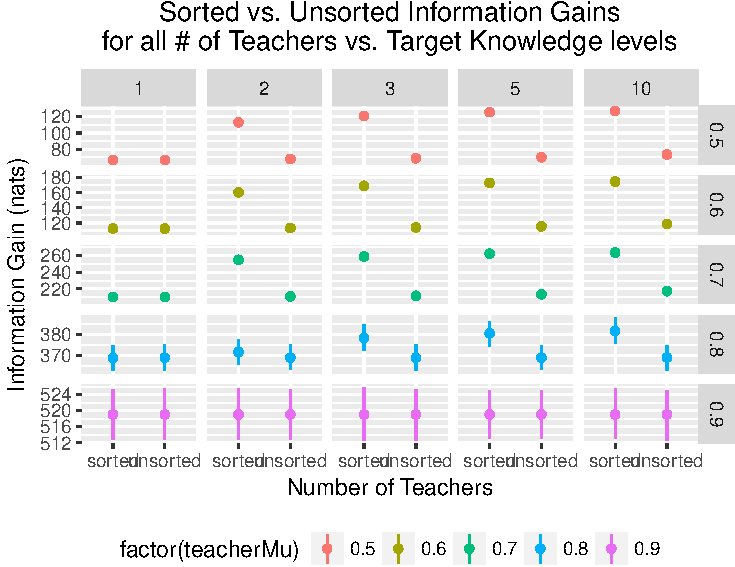
\includegraphics[width=3.25in,height=2.6in]{figs/unnamed-chunk-2-1}
\textbackslash{}caption{[}Student information gain, plotted by target
concept and number of teachers in the school{]}\{Student information
gain, plotted by target concept and number of teachers in the school.
Information gain represents the gain when students are sorted into
classrooms based on knowledge compared with an unsorted baseline. Error
bars show 95\% confidence intervals by non-parametric
bootstrap.\}\label{fig:unnamed-chunk-2} \textbackslash{}end\{figure\}
\textbackslash{}end\{CodeChunk\}

In our first simulation, we explored the effects of grouping students by
their \emph{true prior beliefs} (admins with perfect knowledge), so that
teachers can tailor the examples they teach to that particular group.
This simulation is a replication of results reported in Frank (2014)
using the multi-classroom model developed here. We hypothesized that
sorting students by their true beliefs would increase information gain
compared to random classroom assignment. Our baseline for this
simulation was the unsorted information gain under the same parameters.
For instance, the sorted aggregate IG of a school with 5 teachers and a
target bias of .6 is compared to the unsorted aggregate IG for a school
with 5 teachers and a target bias of .6 using the same school of
students.

Results are shown in Figure 1. Sorted students show greater information
gain than if the same set of students are distributed into unsorted
classrooms. This effect is present for all target concepts but is most
pronounced for less-extreme concepts -- for extreme value concepts
(e.g., a target of .9), almost all students will benefit from seeing the
same examples anyway, rendering sorting irrelevant. Thus, an optimal
school administrator with perfect student knowledge should consistently
opt to sort students into classrooms by their prior beliefs over random
assignment.

\subsection{Simulation 2: Class size}\label{simulation-2-class-size}

\textbackslash{}begin\{CodeChunk\}
\textbackslash{}begin\{figure\}{[}t{]}
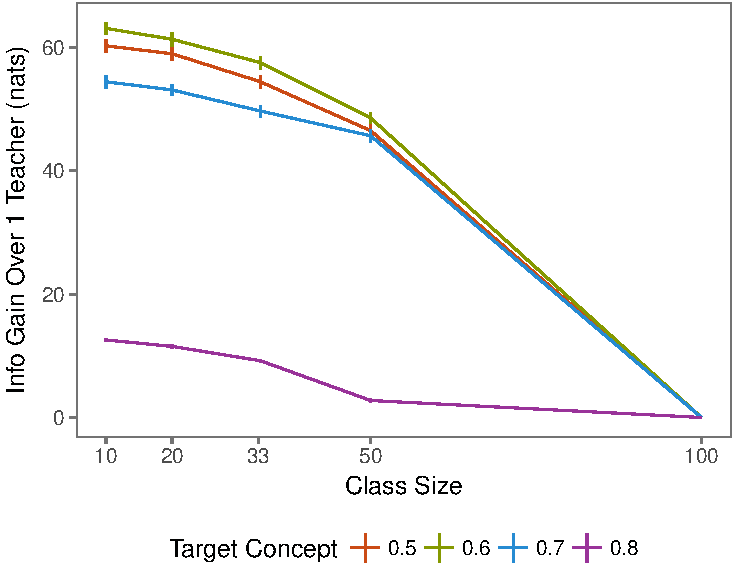
\includegraphics[width=3.25in,height=2.6in]{figs/sim_class_size-1}
\textbackslash{}caption{[}Student information gain, plotted by target
concept and class size{]}\{Student information gain, plotted by target
concept and class size. Information gain represents the gain when
students are sorted into classrooms based on knowledge compared with a
single-classroom baseline. Error bars show 95\% confidence intervals by
non-parametric bootstrap.\}\label{fig:sim_class_size}
\textbackslash{}end\{figure\} \textbackslash{}end\{CodeChunk\}

In our second simulation, again a replication of our prior work, we
explored the effects of adding teachers to the simulated school, leading
to lower class sizes. We hypothesized that increasing the number of
teachers would strictly improve student learning rate (again assuming
perfect knowledge about students): more teachers in a school means that
students are in smaller classes and hence receive better customized sets
of examples from the teacher that appropriately helps students calibrate
their prior beliefs towards the target concept. Our baseline for this
simulation was the sorted information gain under the same target bias
parameters. We observed the predicted pattern (Figure 2), although there
were diminishing returns. After a certain number of teachers, additional
lesson customization becomes less helpful.

\subsection{Simulation 3: Noisy students and
assessments}\label{simulation-3-noisy-students-and-assessments}

\begin{CodeChunk}
\begin{figure*}[t]
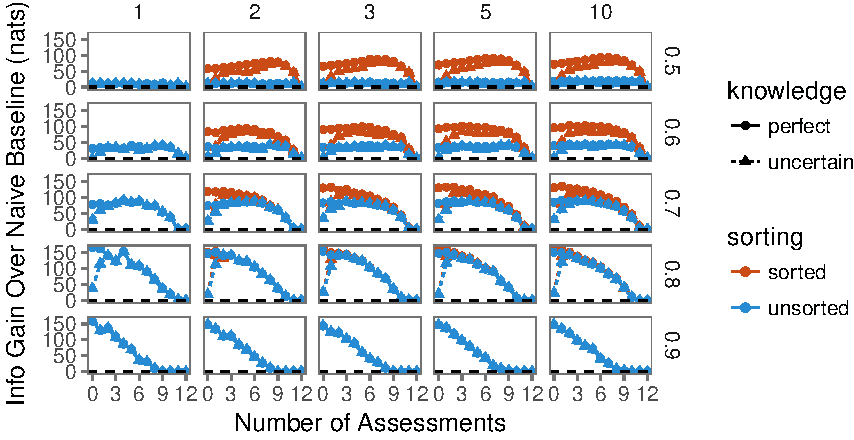
\includegraphics[width=3.25in,height=2.6in]{figs/sim_noisy_students-1} \caption[Information gain plotted by number of assessments (out of 12) for teachers with perfect and uncertain student knowledge]{Information gain plotted by number of assessments (out of 12) for teachers with perfect and uncertain student knowledge. Results shown are for 5 teachers and a target concept of .5.}\label{fig:sim_noisy_students}
\end{figure*}
\end{CodeChunk}

\begin{CodeChunk}
\begin{figure}[t]
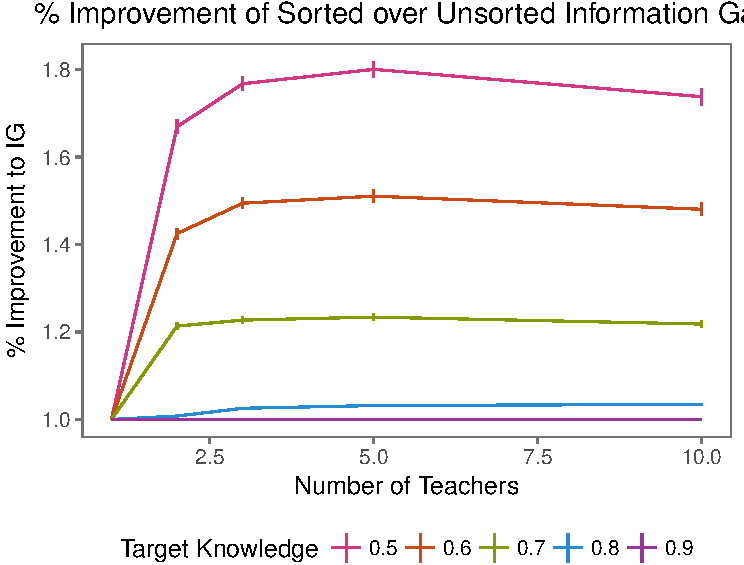
\includegraphics[width=3.25in,height=2.6in]{figs/unnamed-chunk-3-1} \caption[Information gain plotted by number of assessments (out of 12) for teachers with perfect and uncertain student knowledge]{Information gain plotted by number of assessments (out of 12) for teachers with perfect and uncertain student knowledge. Results shown are for 5 teachers and a target concept of .5.}\label{fig:unnamed-chunk-31}
\end{figure}
\begin{figure}[t]
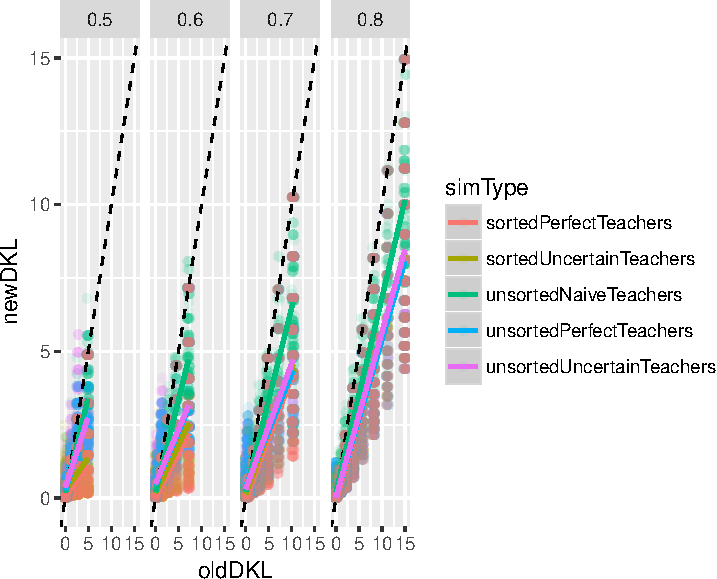
\includegraphics[width=3.25in,height=2.6in]{figs/unnamed-chunk-3-2} \caption[Information gain plotted by number of assessments (out of 12) for teachers with perfect and uncertain student knowledge]{Information gain plotted by number of assessments (out of 12) for teachers with perfect and uncertain student knowledge. Results shown are for 5 teachers and a target concept of .5.}\label{fig:unnamed-chunk-32}
\end{figure}
\end{CodeChunk}

\textbackslash{}begin\{CodeChunk\}
\textbackslash{}begin\{figure\}{[}t{]}
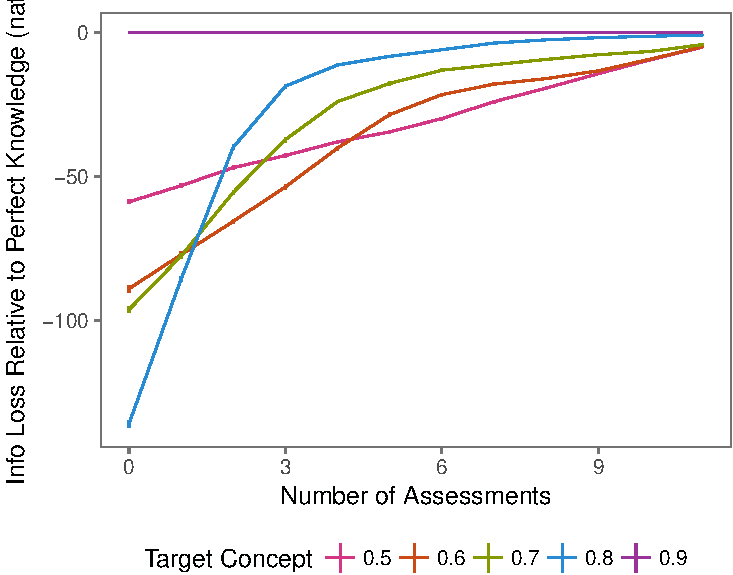
\includegraphics[width=3.25in,height=2.6in]{figs/sim_info_loss-1}
\textbackslash{}caption{[}Student information loss, plotted by target
concept and class size{]}\{Student information loss, plotted by target
concept and class size. Information loss represents loss compared to the
perfect teacher knowledge condition. Error bars show 95\% confidence
intervals by non-parametric bootstrap.\}\label{fig:sim_info_loss}
\textbackslash{}end\{figure\} \textbackslash{}end\{CodeChunk\}

In our third simulation, we relax the assumption that teachers have
perfect knowledge about students. Instead, we assume that the school
faculty starts with a naive uniform representation of the students and
must learn about them via the administration of assessments. In
assessments, students are called upon to demonstrate their knowledge by
sampling from their own distribution. These samples then serve to update
the faculty's estimates of student knowledge. The admin uses these
estimates to sort students into classrooms, and teachers use these
estimates to customize the set of teaching lessons to a particular
student group.

In the simulation, the students have a limited number of learning
opportunities. We found that increasing aggregate IG converges quick
after 10 time steps (noticeable in Figure 5), so we report results with
an arbitrarily chosen 12 time steps. Each assessment or lesson takes 1
time step, and all assessments come before all lessons.

We hypothesized that the noisy students will produce less information
gain than if the faculty had perfect knowledge of student beliefs. We
suspect the school design will differ from the optimal configurations at
two stages: the sorting stage (classrooms will not have maximal
homogeneity), and the teaching stage (the examples selected by any given
teacher will not maximize IG for the students assigned to their class).
Nevertheless, we still believe the improvements to IG by increasing the
number of teachers and reducing class sizes would persist for noisy
students.

We further hypothesized that the optimal use of the allotted time steps
would involve a small or moderate number of assessments and a moderate
to large number of lessons. We thought that a few assessments would get
the estimated beliefs about student knowledge close enough to the
students' true beliefs to minimize sorting errors, leaving teachers with
enough time to teach lessons to move the students' actual beliefs
towards the target concept. Too many assessments would reduce the amount
of time teachers have to teach regardless of how precise their estimates
of student knowledge are; too few assessments would prevent teachers
from selecting helpful examples in their lessons.

Indeed, we found a quadratic shape in the relationship between number of
assessments and aggregate IG. Assessing students helps improve learning
rate by giving teachers better estimates of their beliefs, but they
still need time to subsequently teach towards the target concept.
Additionally, like previous simulations, this effect was most pronounced
in moderate target concepts. These results make intuitive sense.
Teaching concepts where there may be greater variance in student
knowledge relative to each other (e.g.~teaching concepts of .5) demand
more customization in lesson plans with students exhibiting different
levels of mastery.

We hypothesized that a small or moderate number of assessments will be
helpful, outweighing

\subsection{Simulation 4: Pareto frontier with imposed budget
constraints
(TODO)}\label{simulation-4-pareto-frontier-with-imposed-budget-constraints-todo}

\begin{CodeChunk}

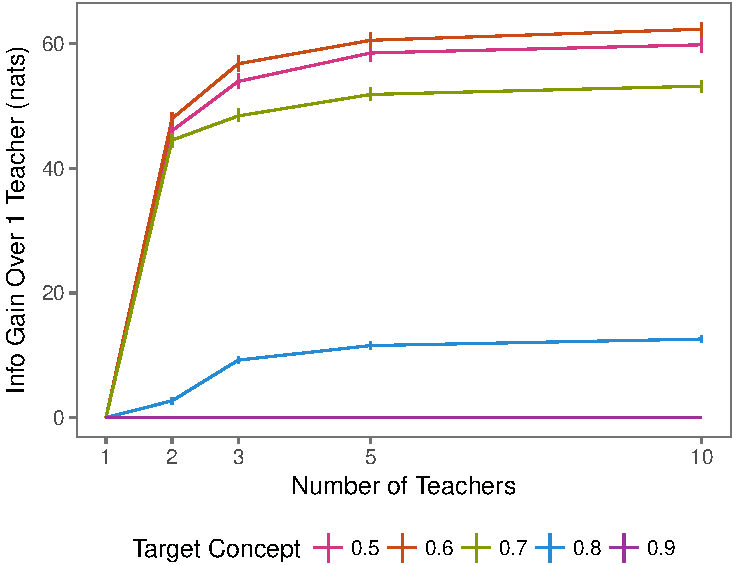
\includegraphics[width=3.25in,height=2.6in]{figs/unnamed-chunk-6-1} \end{CodeChunk}

We hypothesized that for a particular budget constraint and fixed costs
of teachers and assessment, there will be a Pareto frontier of possible
allocations of that budget towards teachers and assessments on which
there will be an optimal allocation that maximizes student learning.
Furthermore, we hypothesized that the individual results about number of
teachers number of assessments would hold within levels of the other.
This is the unification of all previous simulations into one model that
allows us to introduce a real-world constraint of budget.

In this simulation, we test all integer combinations of number of
teachers between 1 and 10 with number of assessments between 0 and 5. We
assigned the cost of each teacher to be CT = \$10 and the cost of each
assessment CA = \$20.

Our baselines were the worst-performing within-target setup. This always
happened to be the 1-teacher 0-assessment setup, which is consistent
with existing education literature, since a single teacher cannot
significantly differentiate learning, and still has a lot of uncertainty
about student beliefs because no assessments are performed.

Our simulated findings support our hypothesis. There is con- siderable
support for an interaction model between teachers, assessments, and the
target bias, F(7, 112) = 48.61, p\textless{}.001. To visualize the
pareto frontier, we draw a heatmap of scores

above baseline along teacher and assessment axes. We con- tinue to see
that the effects continue to be weaker for more extreme learning
concepts, t(294) = -11.09, p\textless{}.001. This result can be seen in
Figure 5.

Since real-world learning concepts are essentially non- negotiable, the
effectiveness of a particular allocation of bud- get should be judged
within-target, i.e.~an optimal setup within the target bias = 0.8 level
should not be penalized for being ineffective in comparison to the
optimal setup for teaching a target bias of 0.5. We normalized the
information gain above baseline within each target bias level. The
results can be seen in 6

Consistent with Simulation 3, increasing the number of assess- ments on
average improves learning rate up until you cannot afford any more
assessments, across all levels of teachers and target biases. Consistent
with Simulation 2, increasing the number of assessments improves
learning rate up until you cannot afford any more assessments, across
all levels of assessments and target biases of 0.5, 0.6, and 0.7.

An interesting result, however, is that having noisy students diminishes
the effectiveness of increasing the number of teach- ers at certain a
target bias of 0.8. While we aren't sure of the specific mechanism by
which this happens, we suspect that having more teachers introduces
additional risk of wrongly sorting students' prior beliefs, which would
increase the het- erogeneity of classrooms. Since a target belief of 0.8
is a possible target belief to show precisely with 5 examples (the basis
of our simulations) but also extreme enough that most students's prior
belief will fall on one side of that target, in- creasing the number of
teachers might actually reduce the effectiveness of the teacher's choice
of examples. A novel finding that emerged not described in existing
educa- tion literature is that there are different patterns of
optimality along the pareto frontiers. As the extremity of the target
bias moves from 0.5 to 0.7, we see that the IG-optimal allocation of
budget shifts from about 5-6 teachers and 2 assessments towards more
assessments at the expense of the number of teachers.

\section{Discussion (TODO)}\label{discussion-todo}

Overall, we were able to replicate many real-world findings from
education literature. We found the sorting students into ability level
classrooms, increasing assessment, and decreasing class size all
increase information gain.

One of the more interesting findings was the influence of the target
bias on the effects we were finding. Based on our results, target bias
significantly moderates each of the effects we found. When teaching an
extremely difficult (or easy, given symmetry) learning concept such that
all student prior beliefs are on one side of the concept, the payoffs to
information gain that sorting, class sizes, and assessment have diminish
because regardless of the level of noise, teachers have relative
certainty about the students' relative level of understanding.
Similarly, target biases that are very close to central (around 0.5)
have a lot to gain from diminishing noise in the system.

Finally, we found that the relative effectiveness of number of teachers
and and the number of assessments varies depend- ing on the target
learning concept. We saw that the most optimal distribution of budget on
the pareto frontier shifted towards reducing student noise when the
target bias was more extreme--this seemed consistent with intuition,
since having more teachers doesn't allow them to better select examples
if the administrator produces greater sorting errors, resulting in
heterogeneous classrooms where each teacher has less cer- tainty about
whether their examples will be useful for any particular student or not.

While a lot of aspects of school learning (peer effects, social
dynamics, etc.) are not built into our model and would be difficult to
capture algorithmically, we believe that there is a lot to be gained
from simulating classroom dynamics. Using stochastic modeling is
particularly useful when exploring the effectiveness of education policy
measures for a handful of reasons. Fundamentally, the merits of
stochastic modeling arise from the use of synthetic data. Since the
studies are computer-simulated, there are no human subjects in the stud-
ies, and all of the data is synthetic. This allows researchers to take
greater liberties in experimental design because there are no ethical
concerns. For instance, we can execute a sim- ulation that will
intentionally misclassify synthetic students into classrooms that are
not appropriate for their achievement level to understand the negative
impact doing so has on both the misclassified student and his peers.
Such a study would not be ethically permissible in an actual school.

Furthermore, no two schools are the same, and the use of mod- eling and
synthetic data enables rapid iteration over different simulated schools
with different simulated students. We can quickly test whether the
purported benefit to student learning of various education interventions
holds with, for example, a limited budget, or highly varied student
achievement levels, or immensely large class sizes. There is also no
risk of student subject attrition that may jeopardize real-world school
studies; synthetic students do not exhibit unpredictable absenteeism,
transfer schools, take sick days, etc. As such, we can cus- tomize our
interventions based on school parameters, validate the robustness of our
results, and better infer generalized find- ings about education policy
without incurring astronomical experimental monetary costs nor require
lengthy longitudinal study. With a complete stochastic model, we can
quickly scale the number of hypotheses we test and the variety of
schools we test them on. Our series of simulations are designed to
replicate real-world results from education literature in a
quantitative, simulated fashion. The first few simulations looked at a
lot of existing educational theory in isolation, while our final
simulation attempts to unify these different design aspects of a school
system into a more holistic view. We found that increasing the number of
teachers (and thus decreasing class size) and increasing the amount of
assessment to improve precision about student beliefs increases student
learning, as predicted in real-world school studies.

Importantly, we were able to generate pareto frontiers allo- cating a
fixed shared resource of budget into the dimensions of teachers and
sorting. The ability to make sense of the tradeoffs that school
administrators and policymakers need to make when designing their
schools can help improve educa- tion. This would be particularly
impactful in communities of low socioeconomic status where academic
achievement tends D to be lower because budgets are particularly
constrained and attracting teaching staff is difficult.

Some of the limitations of the present work is in the assump- tions that
we make to build our model. Most obvious is the simplicity of the
learning task we described during the intro- duction. Most real-world
learning tasks are more complicated and may have multiple objectives.
Furthermore learning in the real-world is affected by a lot of more
abstract facets: peer learning and social environment, parenting styles,
stereotype threat, among other things. These are not captured in the
model, and would be difficult to capture in any model. The agnostic
prior beliefs we 1) use for teachers to generate examples from; 2)
generate student prior beliefs from; and 3) create target bias
distributions with are all uniform distri- butions. These are not
necessarily the case. Respectively, 1) teachers may have prior beliefs
about which examples are more effective, akin to pedagogical knowledge
or pedagogical content knowledge (Cochran, 1991); 2) students may tend
towards certain common prior beliefs/misconceptions about a particular
learning concept; 3) more extreme learning concepts may be more rare,
and thus the admin should weight more heavily the pareto frontier of
moderate target bias values.

\section{Acknowledgements}\label{acknowledgements}

This work supported by NSF BCS \#1456077.

\section{References}\label{references}

\setlength{\parindent}{-0.1in} \setlength{\leftskip}{0.125in} \noindent

\hypertarget{refs}{}
\hypertarget{ref-cover2012}{}
Cover, T. M., \& Thomas, J. A. (2012). \emph{Elements of information
theory}. John Wiley \& Sons.

\hypertarget{ref-frank2014}{}
Frank, M. C. (2014). Modeling the dynamics of classroom education using
teaching games. In \emph{CogSci}.

\hypertarget{ref-frank2012}{}
Frank, M. C., \& Goodman, N. D. (2012). Predicting pragmatic reasoning
in language games. \emph{Science}, \emph{336}(6084), 998--998.

\hypertarget{ref-fuchs1986}{}
Fuchs, L. S., \& Fuchs, D. (1986). Effects of systematic formative
evaluation: A meta-analysis. \emph{Exceptional Children}.

\hypertarget{ref-goodman2016}{}
Goodman, N. D., \& Frank, M. C. (2016). Pragmatic language
interpretation as probabilistic inference. \emph{Trends in Cognitive
Sciences}, \emph{20}(11), 818--829.

\hypertarget{ref-goodman2017}{}
Goodman, N. D., \& Stuhlmüller, A. (n.d.). The design and implementation
of probabilistic programming languages. Retrieved 2017, from
\url{http://dippl.org}

\hypertarget{ref-sadler1989}{}
Sadler, D. R. (1989). Formative assessment and the design of
instructional systems. \emph{Instructional Science}, \emph{18}(2),
119--144.

\hypertarget{ref-slavin1987}{}
Slavin, R. E. (1987). Ability grouping and student achievement in
elementary schools: A best-evidence synthesis. \emph{Review of
Educational Research}, \emph{57}(3), 293--336.

\hypertarget{ref-slavin1990}{}
Slavin, R. E. (1990). Achievement effects of ability grouping in
secondary schools: A best-evidence synthesis. \emph{Review of
Educational Research}, \emph{60}(3), 471--499.

\hypertarget{ref-tomlinson1999}{}
Tomlinson, C. A. (1999). \emph{The differentiated classroom: Responding
to the needs of all learners}. Association for Supervision \& Curriculum
Development.

\end{document}
